\begin{center}
    \captionof{figure}{Within- and Between-Person Effects of Dichotomous Predictor and Outcome}

    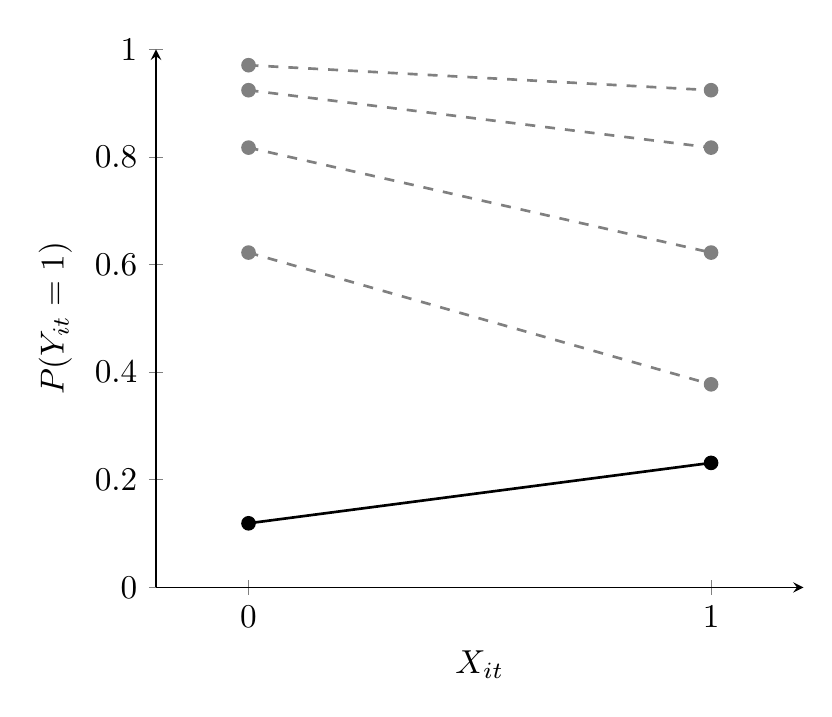
\begin{tikzpicture}[scale=1.2]
    \begin{axis}[
        axis x line=left, 
        axis y line=left, 
        xlabel={$X_{it}$}, ylabel={$P(Y_{it} = 1)$},
        ymin=0, ymax=1, xmin=-0.2, xmax=1.2,
        xtick={0,1}
    ]

    % Define parameters
    \pgfmathsetmacro{\intercept}{-2}  % Logit-scale intercept
    \pgfmathsetmacro{\slopeB}{0.8}     % Between effect in logit space
    \pgfmathsetmacro{\slopeW}{-1}    % Within effect in logit space

    % Compute probabilities for X = 0 and X = 1
    \pgfmathsetmacro{\pBzero}{1 / (1 + exp(-(\intercept)))}
    \pgfmathsetmacro{\pBone}{1 / (1 + exp(-(\intercept + \slopeB)))}

    % Between-person effect (solid black line)
    \addplot[black, thick] coordinates {(0,\pBzero) (1,\pBone)};
    \addplot[black, only marks, mark=*] coordinates {(0,\pBzero) (1,\pBone)};

    % Compute within-person probabilities for X = 0 and X = 1 for different cluster means
    \foreach \shift in {2.5, 3.5, 4.5, 5.5} {
        \pgfmathsetmacro{\pWzero}{1 / (1 + exp(-(\intercept + \shift)))}
        \pgfmathsetmacro{\pWone}{1 / (1 + exp(-(\intercept + \shift + \slopeW)))}

        % Within-person effect (dashed gray line)
        \addplot[gray, thick, dashed] coordinates {(0,\pWzero) (1,\pWone)};
        \addplot[gray, only marks, mark=*] coordinates {(0,\pWzero) (1,\pWone)};
    }

    \end{axis}
\end{tikzpicture}

    \label{fig:withinbetween-binxy}
    \begin{figurenote}
        The solid black slope represents the between-person effect and the dashed solid grey slopes the within-cluster effects. The X-axis simultaneously represents $X_{it}$ for the within-slope and $\mu_{X,i}$ for the between-slope.
    \end{figurenote}
\end{center}


